\section{Schieflastversuch}
Bei diesem Versuch wurde untersucht, wie sich eine unsymmetrische unterspannungsseitige Belastung auf den Betriebszustand des Transformators auswirkt (Messschaltung siehe Abbildung\;\ref{fig:Schieflast_Messschaltung}). In der Praxis treten unsymmetrische Belastungen auf, wenn ein- oder zweiphasige Verbraucher vom Transformator gespeist werden. 
\begin{figure}[ht]
    \centering
    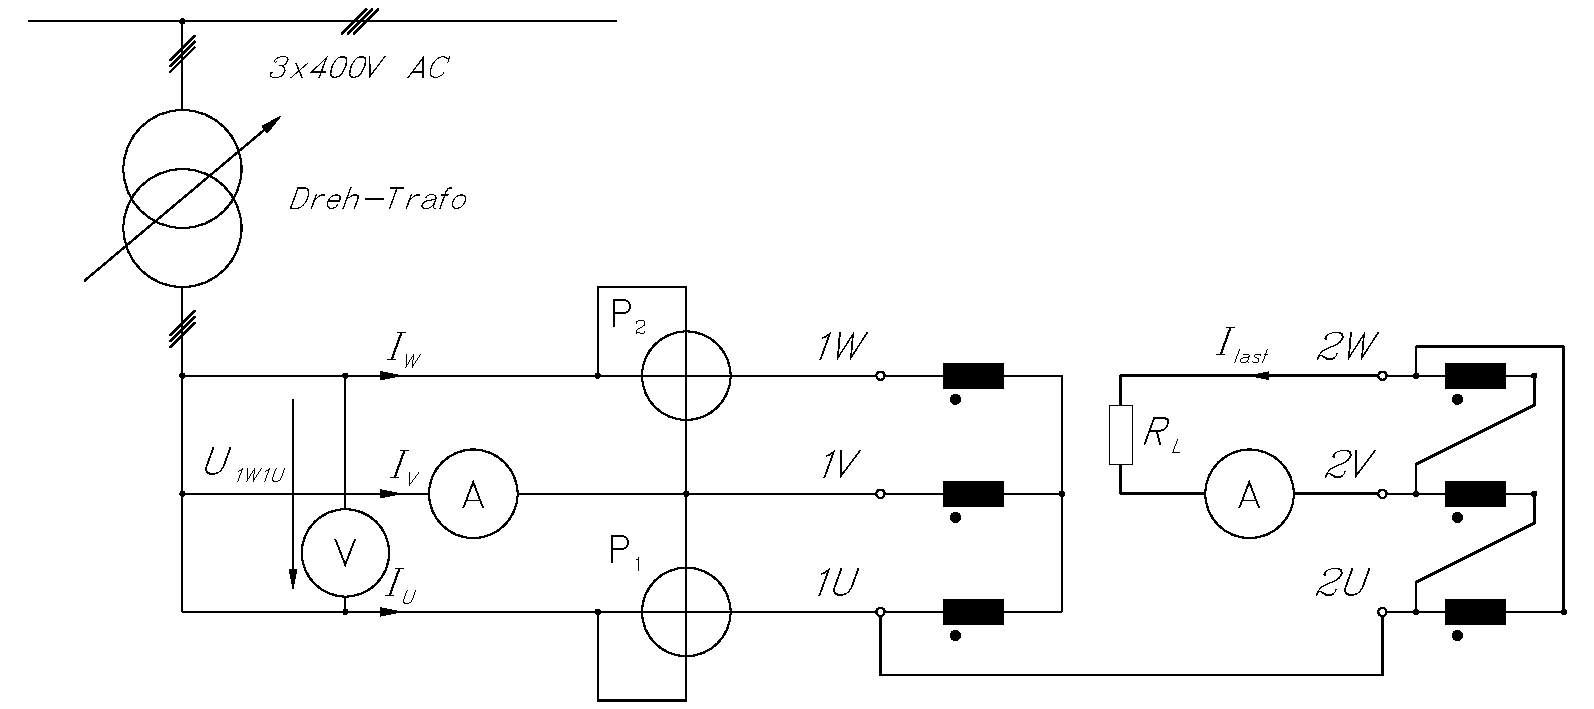
\includegraphics[width=0.75\textwidth]{\currfiledir images/Schieflast}
    \caption{Messschaltung zur Erfassung des Betriebszustandes des 3-Phasen-Transformators bei unsymmetrischer, 2-strängiger, ohmscher Belastung.}
    \label{fig:Schieflast_Messschaltung}
\end{figure}
\noindent
Für den Versuch kann im Allgemeinen entweder der Nullleiter belastet werden (einphasig, einsträngig) oder die Last zwischen zwei Außenleiter geschaltet werden (einphasig, zweisträngig). Für den Fall einer \textbf{Yd}-Schaltung ist kein sekundärseitiger Sternpunkt vorhanden, also wurde der Lastwiderstand $R_L$ zwischen zwei Außenleiter (2W - 2V) geschaltet. 

Die Dreieckwicklung in der \textbf{Yd}-Schaltung bewirkt, dass die durch unsymmetrische Belastung bedingten Nullströme als Kreisstrom auf der Sekundärseite fließen können. Dadurch ist der Durchflutungsausgleich der Schenkel gegeben. Das Primärsystem ohne angeschlossenen Sternpunktleiter muss keine Nullströme führen, und es kommt zu keiner Verzerrung der Spannungen (und keinen gleichphasigen Nullflüssen in den Schenkeln).

Der Lastwiderstand wurde so gewählt, dass näherungsweise Nennstrom fließt. An dem zur Verfügung stehendem Widerstand wurde ein Wert von $\SI{2.75}{\ohm}$ eingestellt. Das führt zu einem Strom
\begin{equation*}
    I_{Last}=\frac{\SI{253}{\volt}}{\SI{2.75}{\ohm}} = \SI{92}{\ampere},
\end{equation*}
was etwa $80\%$ des Nennstromes entspricht.
Die gemessenen Werte sind in \tab{tab:schieflast_1} angeführt.
Es wurden primärseitig die Außenleiterspannungen, die Strangströme und zwei Wirkleistungen für die 2-Wattmeter-Methode gemessen. Sekundärseitig wurde der Strom $I_{Last}$ durch den Widerstand gemessen.
\begin{table}[h!]
    \centering% Tabelle zu leerlauf.csv
    \begin{tabular}{|c|c|c|c|c|c|c|c|c|}
    \hline
    \bfseries $U_{UV}[\SI{}{\volt}]$ & \bfseries $I_U[\SI{}{\ampere}]$ & \bfseries $P_{UV}[\SI{}{\watt}]$ 
    & \bfseries $I_V[\SI{}{\ampere}]$ & \bfseries $U_{UW}[\SI{}{\volt}]$ & \bfseries $U_{WV}[\SI{}{\volt}]$ 
    & \bfseries $I_W[\SI{}{\ampere}]$ & \bfseries $P_{WV}[\SI{}{\watt}]$ & \bfseries $I_{Last}[\SI{}{\ampere}]$
    \csvreader[head to column names]{5/schieflast_1.csv}{}  
    {\\\hline\csvcoli& \csvcolii& \csvcoliii& \csvcoliv& \csvcolv& \csvcolvi& \csvcolvii& \csvcolviii& \csvcolix}
    \\\hline
    \end{tabular}
    \caption{Messwerte zum Schieflastversuch}
    \label{tab:schieflast_1}
\end{table}
\noindent Aus den gemessenen Leistungen errechnet sich die Gesamt-Wirkleistung zu
\begin{equation*}
    P_{ges}=P_{UV}+P_{WV}=\SI{21.7}{\kilo\watt}.
\end{equation*}
% Die Scheinleistung ergibt sich zu
% \begin{equation*}
%     S=
% \end{equation*}
\noindent Die gemessenen gegenseitigen Spannungen zwischen Primär- und Sekundärseite sind in \tab{tab:schieflast_2} angeführt.


\input{\currfiledir schieflast}

\begin{table}[h!]
    \centering% Tabelle zu leerlauf.csv
    \begin{tabular}{|c|c|}
    \hline
    \bfseries  $U_{1U2U}$& \bfseries $0.3$
    \csvreader[]{5/schieflast_2.csv}{}
    {\\\hline\csvcoli& \csvcolii}
    \\\hline
    \end{tabular}
    \caption{Messwerte zur Bestimmung des Zeigerdiagramms; alle Spannungen in $\SI{}{\volt}$}
    \label{tab:schieflast_2}
\end{table}
Das Zeigerdiagramm in Abb.\;\ref{fig:zeigerdiagramm_schieflast} wurde genauso konstruiert wie im Punkt \ref{sec:3}.
Der sekundärseitige Laststrom fließt aufgrund der Dreieckschaltung nur durch die Wicklung (W).
Das Verhältnis der primären Ströme ist in Abb. \ref{fig:zeigerdiagramm_pri_stroeme} dargestellt. Da an die primärseitige Sternschaltung kein Neutralleiter angeschlossen ist, muss im Sternpunkt immer die Kirchhoff'sche Knotenregel 
\begin{equation*}
    \underline{I}_U + \underline{I}_V + \underline{I}_W = 0
\end{equation*}
erfüllt sein, weshalb auf der Primärseite eine gleichartige Stromaufnahme (nur 1 Wicklung stromdurchflossen) nicht möglich ist. D.h. die Wicklungen $1U$ und $1V$ sind ebenfalls stromdurchflossen und der notwendige Durchflutungsausgleich (durch $2U$ und $2V$) wird durch einen sekundärseitigen Kreisstrom in der Dreieckswicklung ermöglicht. 
